\section{test}%
\label{sec:test}
To make Further observation with a laser, you have to attitude it first. 
First thing to do is to calibrate the current to achieve a population inversion. 
For makeing the laser light visible the laser is pointed to a buisnesscardholder
which is filmed by a ccd sensor.
\begin{figure}[h]
		\centering
		\includegraphics[width=0.8\linewidth]{./build/emissionconstruction.pdf}
		\caption{Buisness Card Plot should be here}
		\label{fig:aufbau}
\end{figure}
To achieve the minimal current to laser by induce emission, aternately the head
knob and side knob position is optimized.
Everythime stimulated emission is produce, current is shutting down power a
little bit. 
So that the last visible induce emission is the minimal laser current. 
A Note for stimulated emission is that the light cone from induced emission is
much brighter and more homegenous than by spontanious Emission.
One Example for induce \ref{fig:induce} and spontanious \ref{fig:spontanious} light cone is shown in picture \ref{fig:emission}.
\begin{figure}[h]
		\centering
		\begin{subfigure}[b]{0.45\textwidth}
				\begin{center}
						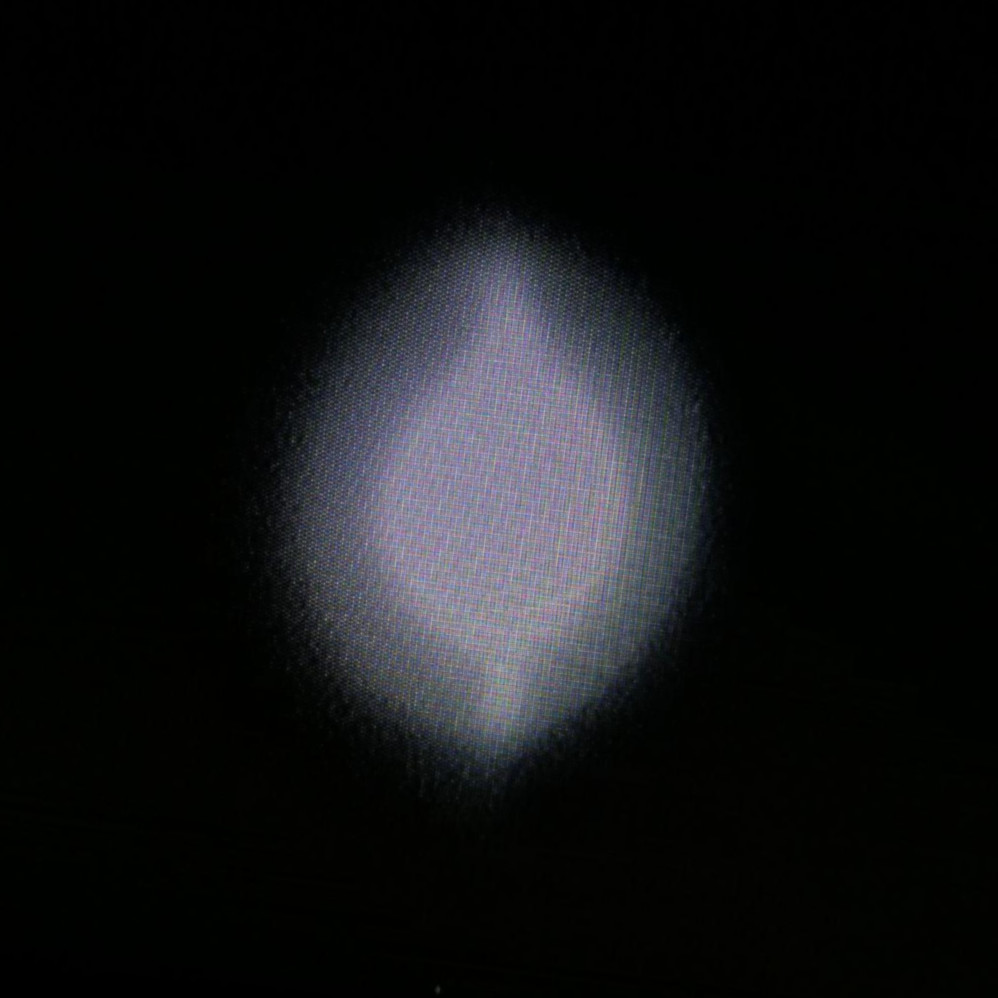
\includegraphics[width=0.9\linewidth]{./content/pictures/below_threshold.jpg}
						\caption{spontanious emission}
				\label{fig:spontanious}
				\end{center}
		\end{subfigure}
		\begin{subfigure}[b]{0.45\textwidth}
				\begin{center}
						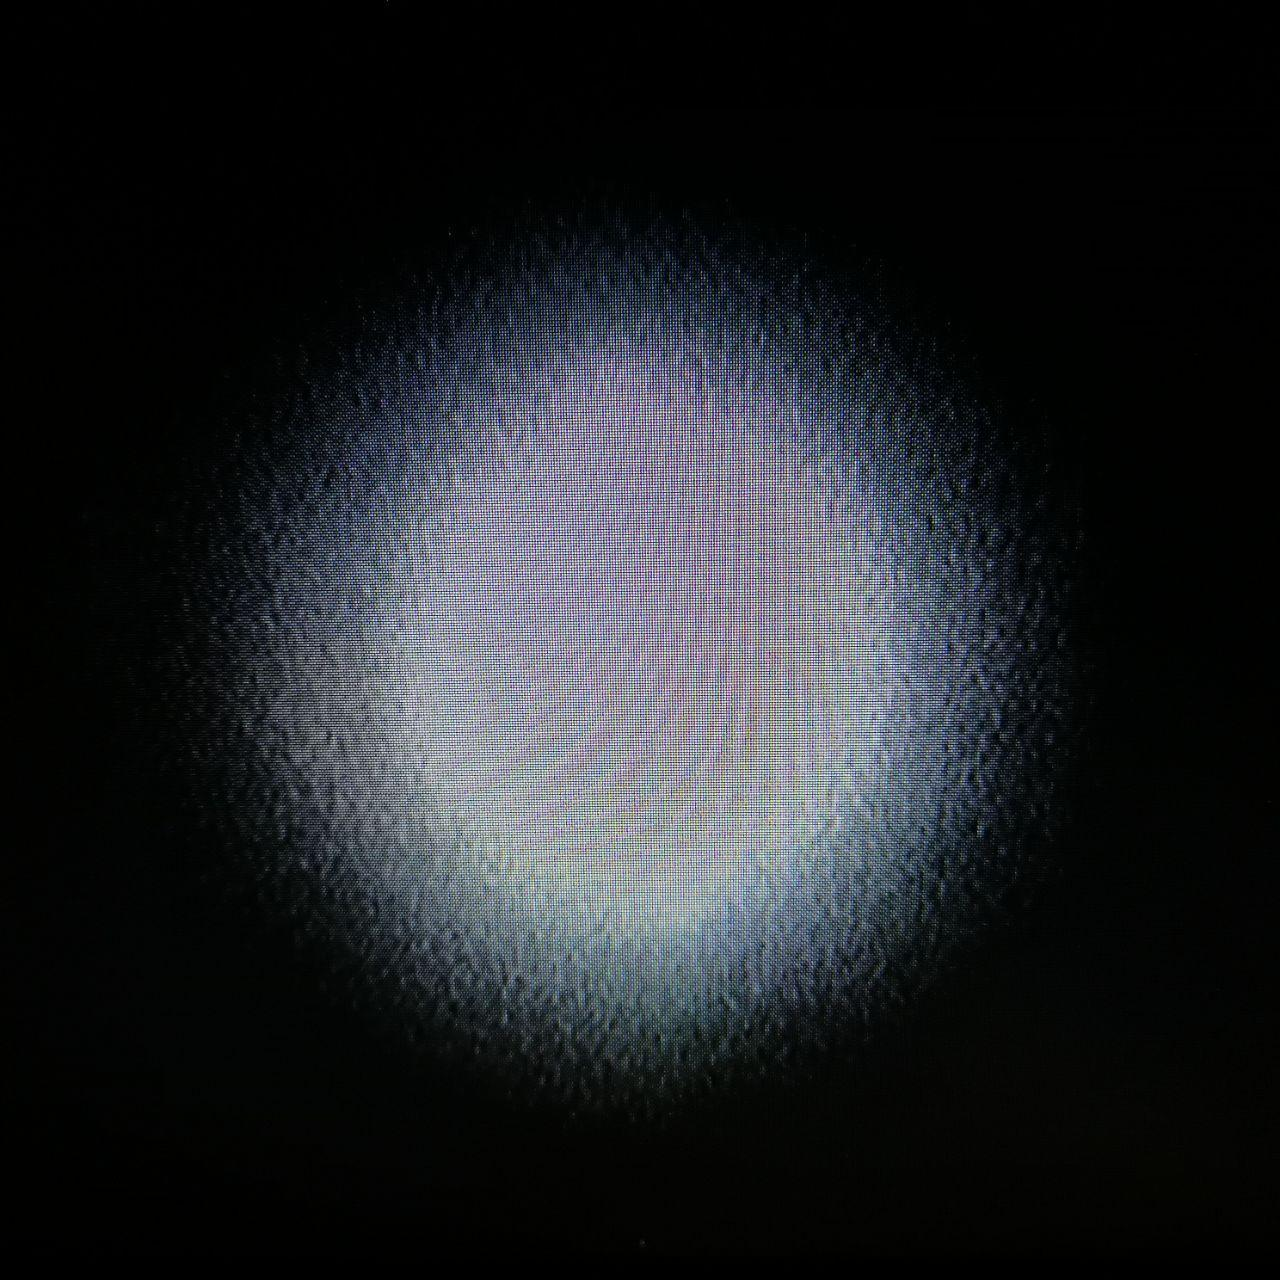
\includegraphics[width=0.9\linewidth]{./content/pictures/above_threshold.jpg}
						\caption{induce emission}
						\label{fig:induce}
				\end{center}
		\end{subfigure}
		% \label{fig:emission}
		\caption{threshold emission}
\end{figure}


\begin{figure}[h]
		\centering
		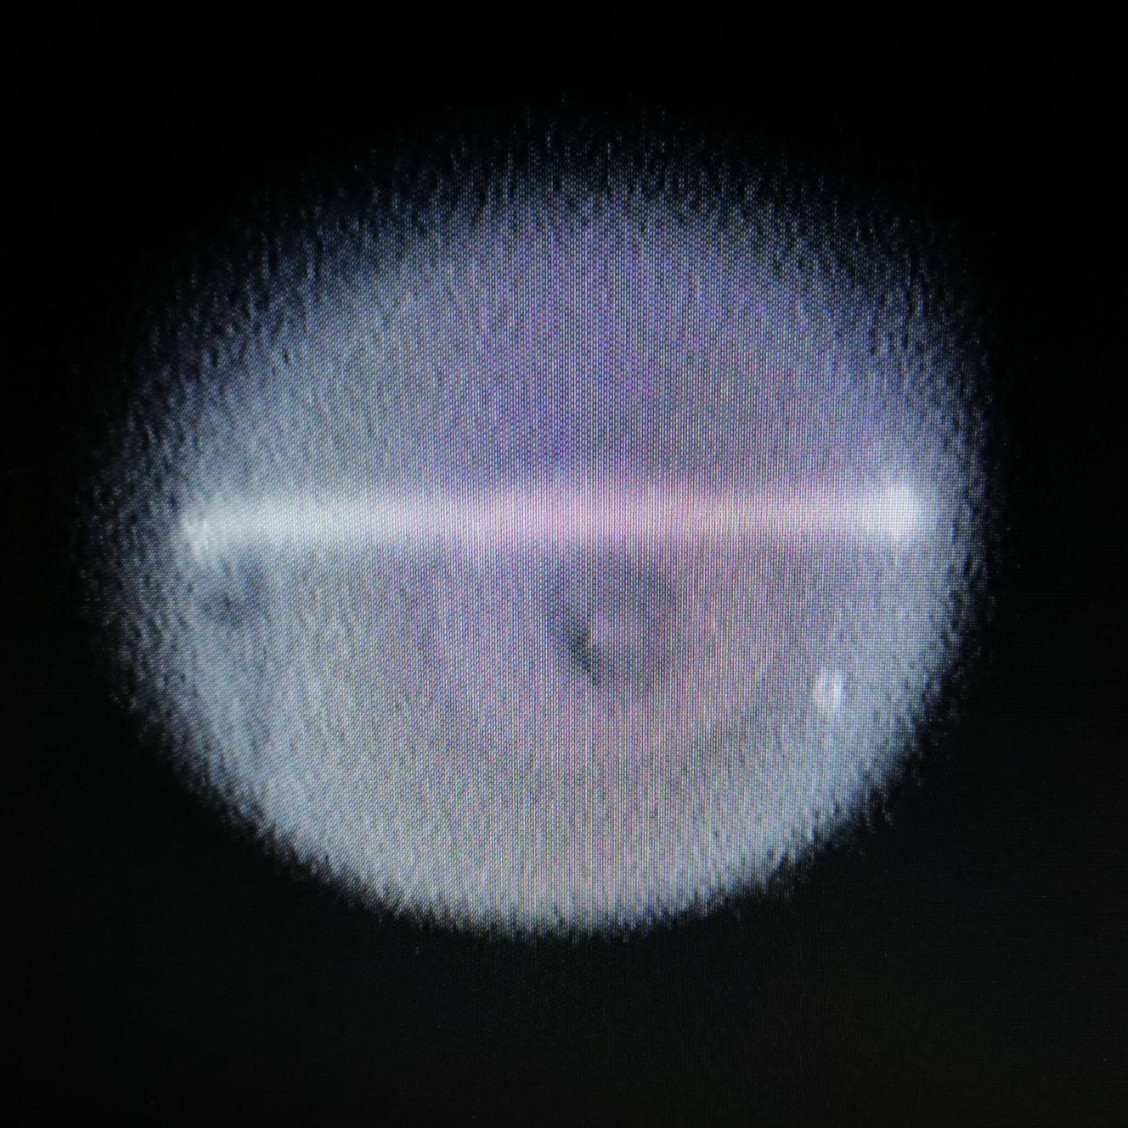
\includegraphics[width=0.4\linewidth]{./content/pictures/fluorescence.jpg}
		\caption{}
		\label{fig:}
\end{figure}

\begin{figure}[h]
		\centering
		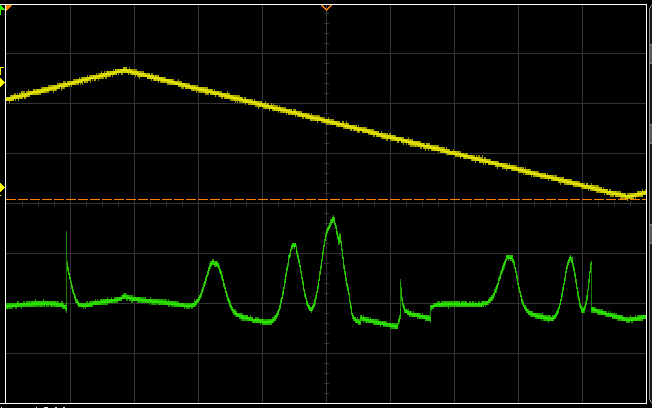
\includegraphics[width=0.8\linewidth]{./content/pictures/scope_136.png}
		\caption{}
		\label{fig:}
\end{figure}

\begin{figure}[h]
		\centering
		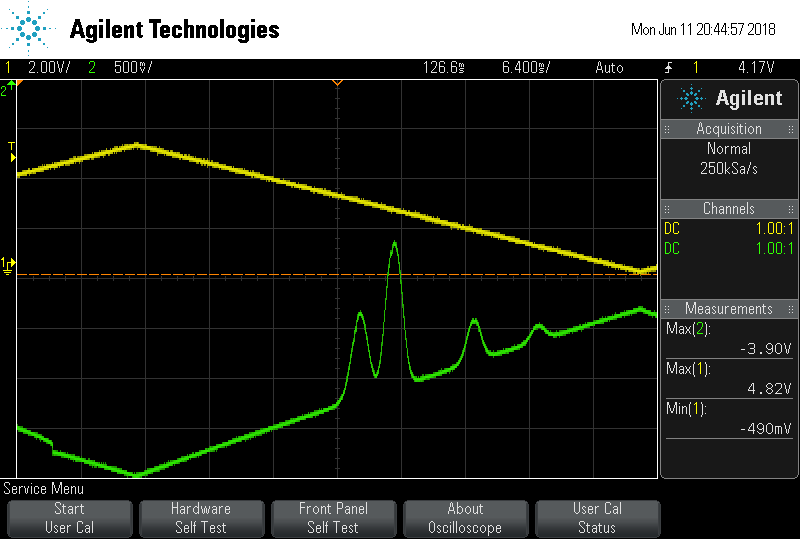
\includegraphics[width=0.8\linewidth]{./content/pictures/scope_139.png}
		\caption{}
		\label{fig:}
\end{figure}

\begin{figure}[ht]
		\centering
		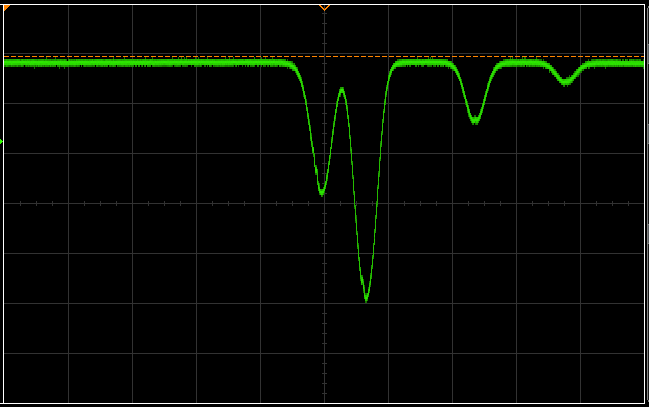
\includegraphics[width=0.8\linewidth]{./content/pictures/scope_140.png}
		\caption{}
		\label{fig:name}
\end{figure}
